\documentclass[11pt,a4paper]{article}
\usepackage{tikz}
\usetikzlibrary{arrows.meta,positioning}
\usepackage{tabularx}
\usepackage{amsmath,amssymb,amsthm}
\usepackage{geometry}
\geometry{margin=1in}
\usepackage{hyperref}
\usepackage{graphicx}
\usepackage{setspace}
\onehalfspacing

\title{\textbf{Paper D-01: Neural Consciousness:\\ A Constraint-Driven Flux Dynamics (CDFD) Perspective}}
\author{Steve Bico Mujjabi, MD\\
\small Independent Researcher\\
\small Founder, Vura Labs\\
\small Kampala, Uganda\\
\small ORCID: 0009-0001-0556-5516}
\date{August 2026}

\begin{document}
\maketitle

% BEGIN SHARED-METHODS POINTER
\noindent\textit{Shared Part IV notation and evidence boundaries are defined in \path{PART_IV_METHODS_AND_CLAIM_BOUNDARY.md}. This paper states only its local observables, comparison, and failure conditions.}
% END SHARED-METHODS POINTER


\begin{abstract}
This paper develops a falsifiable CDFD/AFL model of Neural Consciousness. It maps sensory input, recurrent signaling, metabolic support, and task demand to driving flux $\Phi$, energy, attention, connectivity, inhibition, and integration limits to active constraint $C$, plasticity, arousal, recurrent coordination, and compensatory recruitment to responsiveness $S$, and learned priors, synaptic state, injury, sleep, and developmental history to structural memory $M_s$. The target outcome is integration, reportability, performance, and recovery, tested against neurophysiology, imaging, perturbation, behavior, metabolic data, and longitudinal records. The paper treats universality as a shared model architecture rather than an assertion that unlike systems have the same material mechanism. It states the negative result that would make the mapping unnecessary and places the domain claim inside the cumulative CDFD programme and its reproducible runtime boundary.
\end{abstract}

\section{Introduction}

A human brain consumes 20\% of the body's metabolic energy despite representing only 2\% of its mass. This massive energy expenditure is required to maintain the continuous electrical and chemical flux across billions of synaptic junctions. The brain is not a static computer; it is a highly turbulent fluid of information.

To prevent this immense flux from spiraling into chaotic seizures, the brain deploys massive inhibitory constraints. The interplay between excitatory transmission and inhibitory gating creates the highly ordered, complex patterns we experience as cognition.

\section{The Cognitive Adaptive Surface}
We apply the Adaptive Operating Ratio to neurobiology:
\begin{equation}
    \Psi_s = \left( \frac{\Phi}{C} \right) \cdot S \cdot M_s
\end{equation}

For a specific cortical region:
\begin{itemize}
    \item \textbf{Flux ($\Phi$)}: The rate of excitatory action potentials (e.g., glutamate transmission) and the volume of incoming sensory data.
    \item \textbf{Constraint ($C$)}: The inhibitory tone of the network (e.g., GABAergic interneurons) and the metabolic limits of the astrocytes providing energy.
    \item \textbf{Responsiveness ($S$)}: Neuroplasticity---the capacity of the tissue to rapidly grow new dendritic spines or upregulate receptor density to absorb new information.
    \item \textbf{Memory ($M_s$)}: Long-Term Potentiation (LTP) and structural engrams. The physical reinforcement of a synapse "remembers" past flux, acting as a chronic, semi-permanent modifier to the local topological constraints.
\end{itemize}

\subsection{Epilepsy and PTSD as Topological Failures}
A healthy, conscious brain operates exactly at the edge of criticality ($\Psi_s \approx 1$). The flux is maximal, but perfectly contained by the constraints, allowing complex, ordered thought to propagate.

If the inhibitory constraint $C$ drops abruptly (e.g., due to a chemical imbalance or trauma), the excitatory flux $\Phi$ runs completely unchecked. The adaptive ratio skyrockets ($\Psi_s \gg 1$). The localized region of the brain is overwhelmed, and the unchecked electrical cascade spreads topologically across the cortex. This is an \textbf{Epileptic Seizure}, the neurological equivalent of a supernova or a power grid cascading failure.

Conversely, consider Psychological Trauma (PTSD). A massively terrifying sensory input causes the brain to aggressively enforce a memory lock ($M_s \to 1.0$) on specific amygdala-hippocampal circuits. The brain permanently elevates the constraint $C$ around that specific informational pathway to prevent the traumatic flux from recurring. The local topology becomes rigidly frozen ($\Psi_s \ll 1$). The patient loses cognitive flexibility because the structural memory refuses to adapt to new, safe environments.



\section{Measurement Layer}

% BEGIN PART IV MAJOR CROSS-DOMAIN UPGRADE
\section{Cross-Domain Model Upgrade: Mechanism, Scale, and Tests}

\subsection{Observable Translation}

The paper-specific translation begins with an observable chain rather than a
verbal analogy. For Neural Consciousness, the proposed drive is sensory input, recurrent signaling, metabolic support, and task demand.
The active limitation is energy, attention, connectivity, inhibition, and integration limits. Responsiveness is carried by
plasticity, arousal, recurrent coordination, and compensatory recruitment, while retained state is represented by
learned priors, synaptic state, injury, sleep, and developmental history. The outcome to explain is integration, reportability, performance, and recovery.

\begin{table}[htbp]
\centering
\small
\caption{Operational CDFD/AFL map for Paper D-01.}
\begin{tabularx}{\textwidth}{|l|X|X|}
\hline
\textbf{Term} & \textbf{Paper-specific observable meaning} & \textbf{Measurement question} \\
\hline
$\Phi$ & sensory input, recurrent signaling, metabolic support, and task demand & What rate, load, gradient, or demand enters the focal system? \\
\hline
$C$ & energy, attention, connectivity, inhibition, and integration limits & Which measured bottleneck limits transfer, function, or recovery? \\
\hline
$S$ & plasticity, arousal, recurrent coordination, and compensatory recruitment & Which process changes effective capacity or reroutes the load? \\
\hline
$M_s$ & learned priors, synaptic state, injury, sleep, and developmental history & Which retained state makes equal present loads produce different futures? \\
\hline
$Y$ & integration, reportability, performance, and recovery & Which outcome is predicted out of sample, with uncertainty? \\
\hline
\end{tabularx}
\end{table}

\begin{figure}[htbp]
\centering
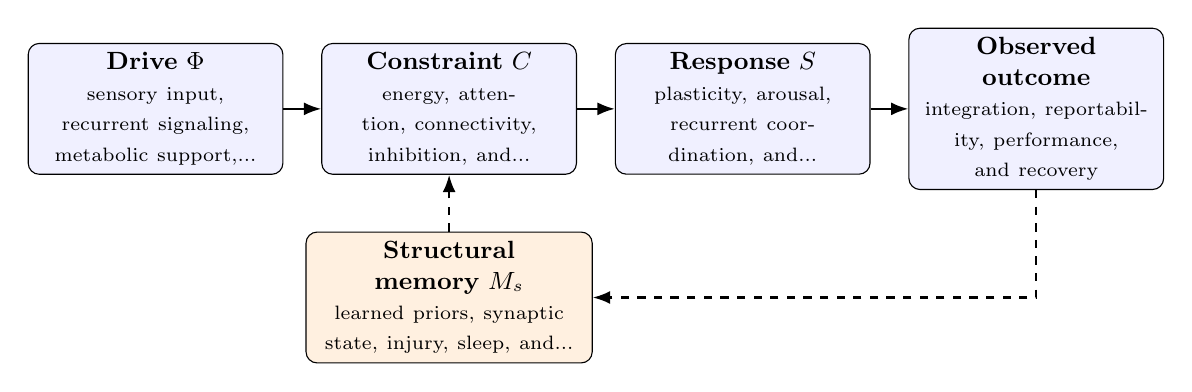
\begin{tikzpicture}[
    node distance=0.48cm,
    every node/.style={font=\small},
    box/.style={draw, rounded corners, align=center, minimum height=1.45cm, text width=3.0cm, fill=blue!6},
    memory/.style={draw, rounded corners, align=center, minimum height=1.25cm, text width=3.4cm, fill=orange!12},
    flow/.style={-{Latex[length=2.2mm]}, thick},
    feedback/.style={-{Latex[length=2.2mm]}, thick, dashed}
]
\node[box] (drive) {\textbf{Drive $\Phi$}\\\scriptsize sensory input, recurrent signaling, metabolic support,...};
\node[box, right=of drive] (constraint) {\textbf{Constraint $C$}\\\scriptsize energy, attention, connectivity, inhibition, and...};
\node[box, right=of constraint] (response) {\textbf{Response $S$}\\\scriptsize plasticity, arousal, recurrent coordination, and...};
\node[box, right=of response] (outcome) {\textbf{Observed outcome}\\\scriptsize integration, reportability, performance, and recovery};
\node[memory, below=0.72cm of constraint] (memory) {\textbf{Structural memory $M_s$}\\\scriptsize learned priors, synaptic state, injury, sleep, and...};
\draw[flow] (drive) -- (constraint);
\draw[flow] (constraint) -- (response);
\draw[flow] (response) -- (outcome);
\draw[feedback] (outcome.south) |- (memory.east);
\draw[feedback] (memory.north) -- (constraint.south);
\end{tikzpicture}
\caption{Paper D-01 observable CDFD/AFL architecture for Neural Consciousness. Solid arrows give the proposed forward chain; dashed arrows make history-dependent feedback explicit.}
\label{fig:d01-architecture}
\end{figure}

\subsection{Paper-Specific Causal Hypothesis}

For this paper, the hypothesized causal sequence is specific. A change in
sensory input, recurrent signaling, metabolic support, and task demand arrives faster than plasticity, arousal, recurrent coordination, and compensatory recruitment can compensate.
This raises or redistributes energy, attention, connectivity, inhibition, and integration limits. If the load persists,
the retained state encoded by learned priors, synaptic state, injury, sleep, and developmental history changes the next response, so a later event of equal
magnitude can produce a different trajectory in integration, reportability, performance, and recovery. The
scientific task is to estimate that sequence against the best ordinary model of
the domain, not merely to redescribe the outcome after it occurs.

\subsection{Cross-Scale Translation Without Mechanistic Erasure}

For the domain applications family, the cross-domain translation is a disciplined test across systems with very different material mechanisms. A valid mapping preserves the baseline science of the domain, declares the scale of every variable, and earns its place through a discriminating prediction rather than resemblance alone. \cite{Holling1973,Turing1952,Shannon1948,BakTangWiesenfeld1987}
The required scale declaration for this paper is milliseconds to lifetimes; synapses to whole-brain networks. At short
scales, the key question is whether the incoming drive is transmitted,
buffered, or diverted. At intermediate scales, response changes effective
capacity and network exposure. At long scales, retained structure can alter the
state space itself. A result is genuinely cross-scale only when the aggregation
rule is stated and the same conclusion is not an artifact of averaging.

\subsection{Evidence Ladder and Discriminating Tests}

\begin{table}[htbp]
\centering
\small
\caption{Evidence ladder for Paper D-01. Each rung can fail independently.}
\begin{tabularx}{\textwidth}{|p{0.17\textwidth}|X|X|}
\hline
\textbf{Test} & \textbf{Design} & \textbf{Discriminating result} \\
\hline
Proxy audit & Measure neurophysiology, imaging, perturbation, behavior, metabolic data, and longitudinal records and preregister how each record maps to $\Phi$, $C$, $S$, $M_s$, and $Y$. & The mapping fails if proxies are non-identifiable, circular, or change meaning across cases. \\
\hline
Load ramp & Apply or observe a controlled perturbation of arousal, connectivity, or sensory load while estimating the dominant constraint and response time. & A threshold claim requires a reproducible nonlinear change and uncertainty bounds, not a visually chosen breakpoint. \\
\hline
Recovery and memory & Match present load across units with different histories, then compare recovery paths. & The memory claim requires history-dependent divergence after current conditions are controlled. \\
\hline
Model comparison & Compare the baseline domain model with and without the CDFD/AFL state variables using held-out data. & The paper's stated falsifier is: CDFD variables do not improve discrimination among competing consciousness models. \\
\hline
\end{tabularx}
\end{table}

\subsection{Research Programme and Boundary Conditions}

The immediate research programme has four steps. First, construct a documented
dataset from neurophysiology, imaging, perturbation, behavior, metabolic data, and longitudinal records and retain raw units before normalization.
Second, fit a baseline domain model and report its calibration and out-of-sample
error. Third, add the smallest identifiable CDFD/AFL state extension and test
whether it improves prediction of integration, reportability, performance, and recovery. Fourth, repeat the
analysis across the declared scale range and publish negative cases as part of
the cross-domain translation audit.

% END PART IV MAJOR CROSS-DOMAIN UPGRADE

\section{Conclusion}
Consciousness is the experiential artifact of a system actively regulating its own information flow at the edge of thermodynamic criticality. By understanding the brain as an active CDFD surface, psychiatric and neurological disorders cease to be arbitrary chemical imbalances and instead reveal themselves as highly predictable topological phase failures.
\section*{Conflict of Interest} The author declares no conflict of interest.
\section*{Data Availability}
Part-specific runtime diagnostics are under each Part's \path{outputs/} directory.

Release-wide code: \path{Part_E_Synthesis/supplementary/}.

Generated summaries: \path{Part_E_Synthesis/outputs/}.

Figures: \path{Part_E_Synthesis/figures/}.


\section{Reference Layer}
\bibliographystyle{plain}
\bibliography{universal_afl_references}
\end{document}
